\chapter{Conclusion}

\begin{theorem}[Loi faible des grands nombres]
 Soit $(X_n)_{n \in \boldsymbol{N}}$ une suite de variable aléatoire indépendante et identiquement distribuée de même loi que X (loi mère). Si $\mathbb{E}[|X|] < +\infty$, alors $\overline{X_n} \rightarrow \mathbb{E}[X]$
\end{theorem}


On ne rappele pas la loi faibles des grands nombres pour rien.\\
En effet,elle peut être observée dans les modèles SIR déterministes et stochastiques.\\
Plus précisément,on peut montrer le modèle stochastique converge vers le modèle déterministe correspondant lorsque la taille de la population tend vers l'infini. Ainsi,on peut en conclure que la faible loi des grands nombres est un concept qui fournit une justification mathématique à l'utilisation de modèles déterministes pour approcher le comportement des modèles stochastiques parmi une grande population, tel que pendant une épidémie mondiale.

\begin{figure}[h]
\centering
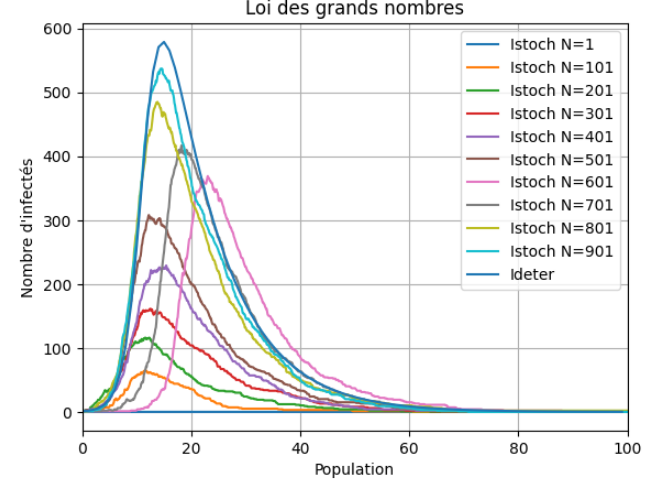
\includegraphics[width=0.5\textwidth]{figs/sir_loi_grands_nombres.png}
\caption{Loi des grands nombres appliqués au modèle stochastique SIR}
\label{fig:loi_grands_nombres}
\end{figure}